\label{chap:methodology}

Será utilizada a linguagem de programação Python, para a extração dos dados através de web scraping realizado em sites que possuem a geolocalização dos empreendimentos dos ativos. Estes sites contém informações de todos FIIs listados na Bolsa de Valores (B3), seus respectivos ativos imobiliários e o histórico de seus rendimentos.

Com os dados extraídos e tratados, o estudo visa criar um mapa do território brasileiro onde estarão dispostos os imóveis dos fundos e suas respectivas localizações representadas por marcadores. Os marcadores serão distinguidos por cores, onde cada cor representará o FII a qual ele pertence e o seu tamanho demonstrará a renda/valorização do fundo. A partir desta visualização o estudo tende a criar um ambiente de maior visualização e análise.

\section{Extração por \emph{Webscrapping}}
\label{sec:extraction_by_webscrapping}
\begin{table}
\begin{centering}
\csvautobooktabular {\tablePath/ImovelPorEstado.csv}
\caption{\label{tab:papers_per_state} Número de ativos de imóveis por estado para os 118 fundos imobiliários analisados.}
\end{centering}
\end{table}

Foi extraído os dados dos fundos imobiliários do site \emph{fundsexplorer}. Excluímos todos os fundos com volume médio igual a zero e com missing values, pois estes podem ter sido incorporado por outros, duplicando assim os ativos.

Obteve-se então uma base de 118 fundos imobiliários no Brasil, destes, 74 tem 390 ativos divididos em 19 estados e 123 cidades.  O resultado final pode ser observado na tabela~\ref{tab:papers_per_state}, ordenada pela quantidade de papeis em cada estado. Notadamente, São Paulo possui grande destaque com 56\% dos ativos, seguido pelo Rio de Janeiro com 17\%. No total, a região sudeste corresponde a 81\% dos ativos.

Após extrair-se as informçães obteve-se o \emph{dataset} de ativos na seguinte estrutura~\ref{tab:example_papers}. Observa-se que esta estrutura contém diversos endereços e em alguns casos múltiplos endereços na mesma linha. Por este motivo, foi necessário tratar-se os dados obtidos, conforme demonstrado na figura~\ref{fig:geoencoding_and_problems}.

\begin{table}
\begin{centering}
%\csvautobooktabular[separator=pipe]{\tablePath/ExemplosAtivos.csv}
\begin{tabular}{l>{\raggedright}p{0.12\textwidth}>{\raggedright}p{0.2\textwidth}>{\raggedright}p{0.15\textwidth}l>{\raggedright}p{0.1\textwidth}>{\raggedright}p{0.12\textwidth}}
\hline 
Fundo & Título & Endereço & Bairro & UF & Cidade & Área(\texttwosuperior{})\tabularnewline
\hline 
ABCP11 & Grand Plaza Shopping & Av. Industrial, 600 & Tamanduateí 3 & SP & Santo André & 69.628\tabularnewline
AEFI11 & Campinas & Avenida John Boyd Dunlop, s/n & Jardim Ipaussurama & SP & Campinas & 96.435,16 \tabularnewline
AEFI11 & Cuiabá & Avenida Fernando Corrêa da Costa, s/nº & Nossa Senhora Aparecida & MT & Cuiabá & 25.000 \tabularnewline
AGCX11 & Ag 14 Bis & Av. Marechal Câmara, 160 & Centro & RJ & Rio de Janeiro & 1.900,31 \tabularnewline
AGCX11 & Ag Av Chile & Av. República do Chile, 230 & Centro & RJ & Rio de Janeiro & 1.139,67 \tabularnewline
AGCX11 & Ag Av. Pres. Wilson & Av. Rio Branco, 311-B & Centro & RJ & Rio de Janeiro & 713,62 \tabularnewline
AGCX11 & Ag Bandeira & R. Mariz e Barros, 79 (Loja) & Praça da Bandeira & RJ & Rio de Janeiro & 1.339 \tabularnewline
AGCX11 & Ag Barra Funda & Av. Rio Branco, 1675 (Loja) & Campos Eliseos & SP & São Paulo & 1.293,02 \tabularnewline
AGCX11 & Ag Benedito Coutinho & R. Antônio Bernardo Coutinho, 163 & Centro & SP & Osasco & 1.206,10 \tabularnewline
AGCX11 & Ag Campo Limpo & Est. do Campo Limpo, 5520 & Vila Pirajussara & SP & São Paulo & 604 \tabularnewline
AGCX11 & Ag Capão Redondo & Estrada de Itapecerica, 3429 & Vila Maracana & SP & São Paulo & 1.448,48 \tabularnewline
AGCX11 & Ag Estrada Rio do A & Est. Rio do A, 1131 &  & RJ & Campo Grande & 571,41 \tabularnewline
AGCX11 & Ag Guaianases & R. Salvador Gianetti, 436 & Guaianases & SP & São Paulo & 2.475,10 \tabularnewline
AGCX11 & Ag Guarapiranga & Av. de Pinedo, 228 & Capela do Socorro & SP & São Paulo & 1.312,18 \tabularnewline
AGCX11 & Ag Hebraica & Av. Brigadeiro Faria Lima, 1644 & Jardim Paulistano & SP & São Paulo & 323,31 \tabularnewline
AGCX11 & Ag Inconfidencia & R. Curitiba, 888 & Centro & MG & Belo Horizonte & 2.373,17 \tabularnewline
\dots{} & \dots{} & \dots{} & \dots{} & \dots{} & \dots{} & \dots{}\tabularnewline
\hline 
\end{tabular}
\caption{\label{tab:example_papers}Exemplos de Ativos extraídos pela utilização de técnicas de \emph{webscrapping}}
\end{centering}
\end{table}

Geocodificamos o endereço dos ativos através do GoogleEarth e obtivos um arquivo .kml. Em sequência, os dados foram importados no software QGis e ao plotar-se os diversos ativos sobre o mapa dos estados da federação obteve-se a figura \ref{fig:papers_vs_dividends}.

\begin{center}
\begin{figure}
\begin{centering}
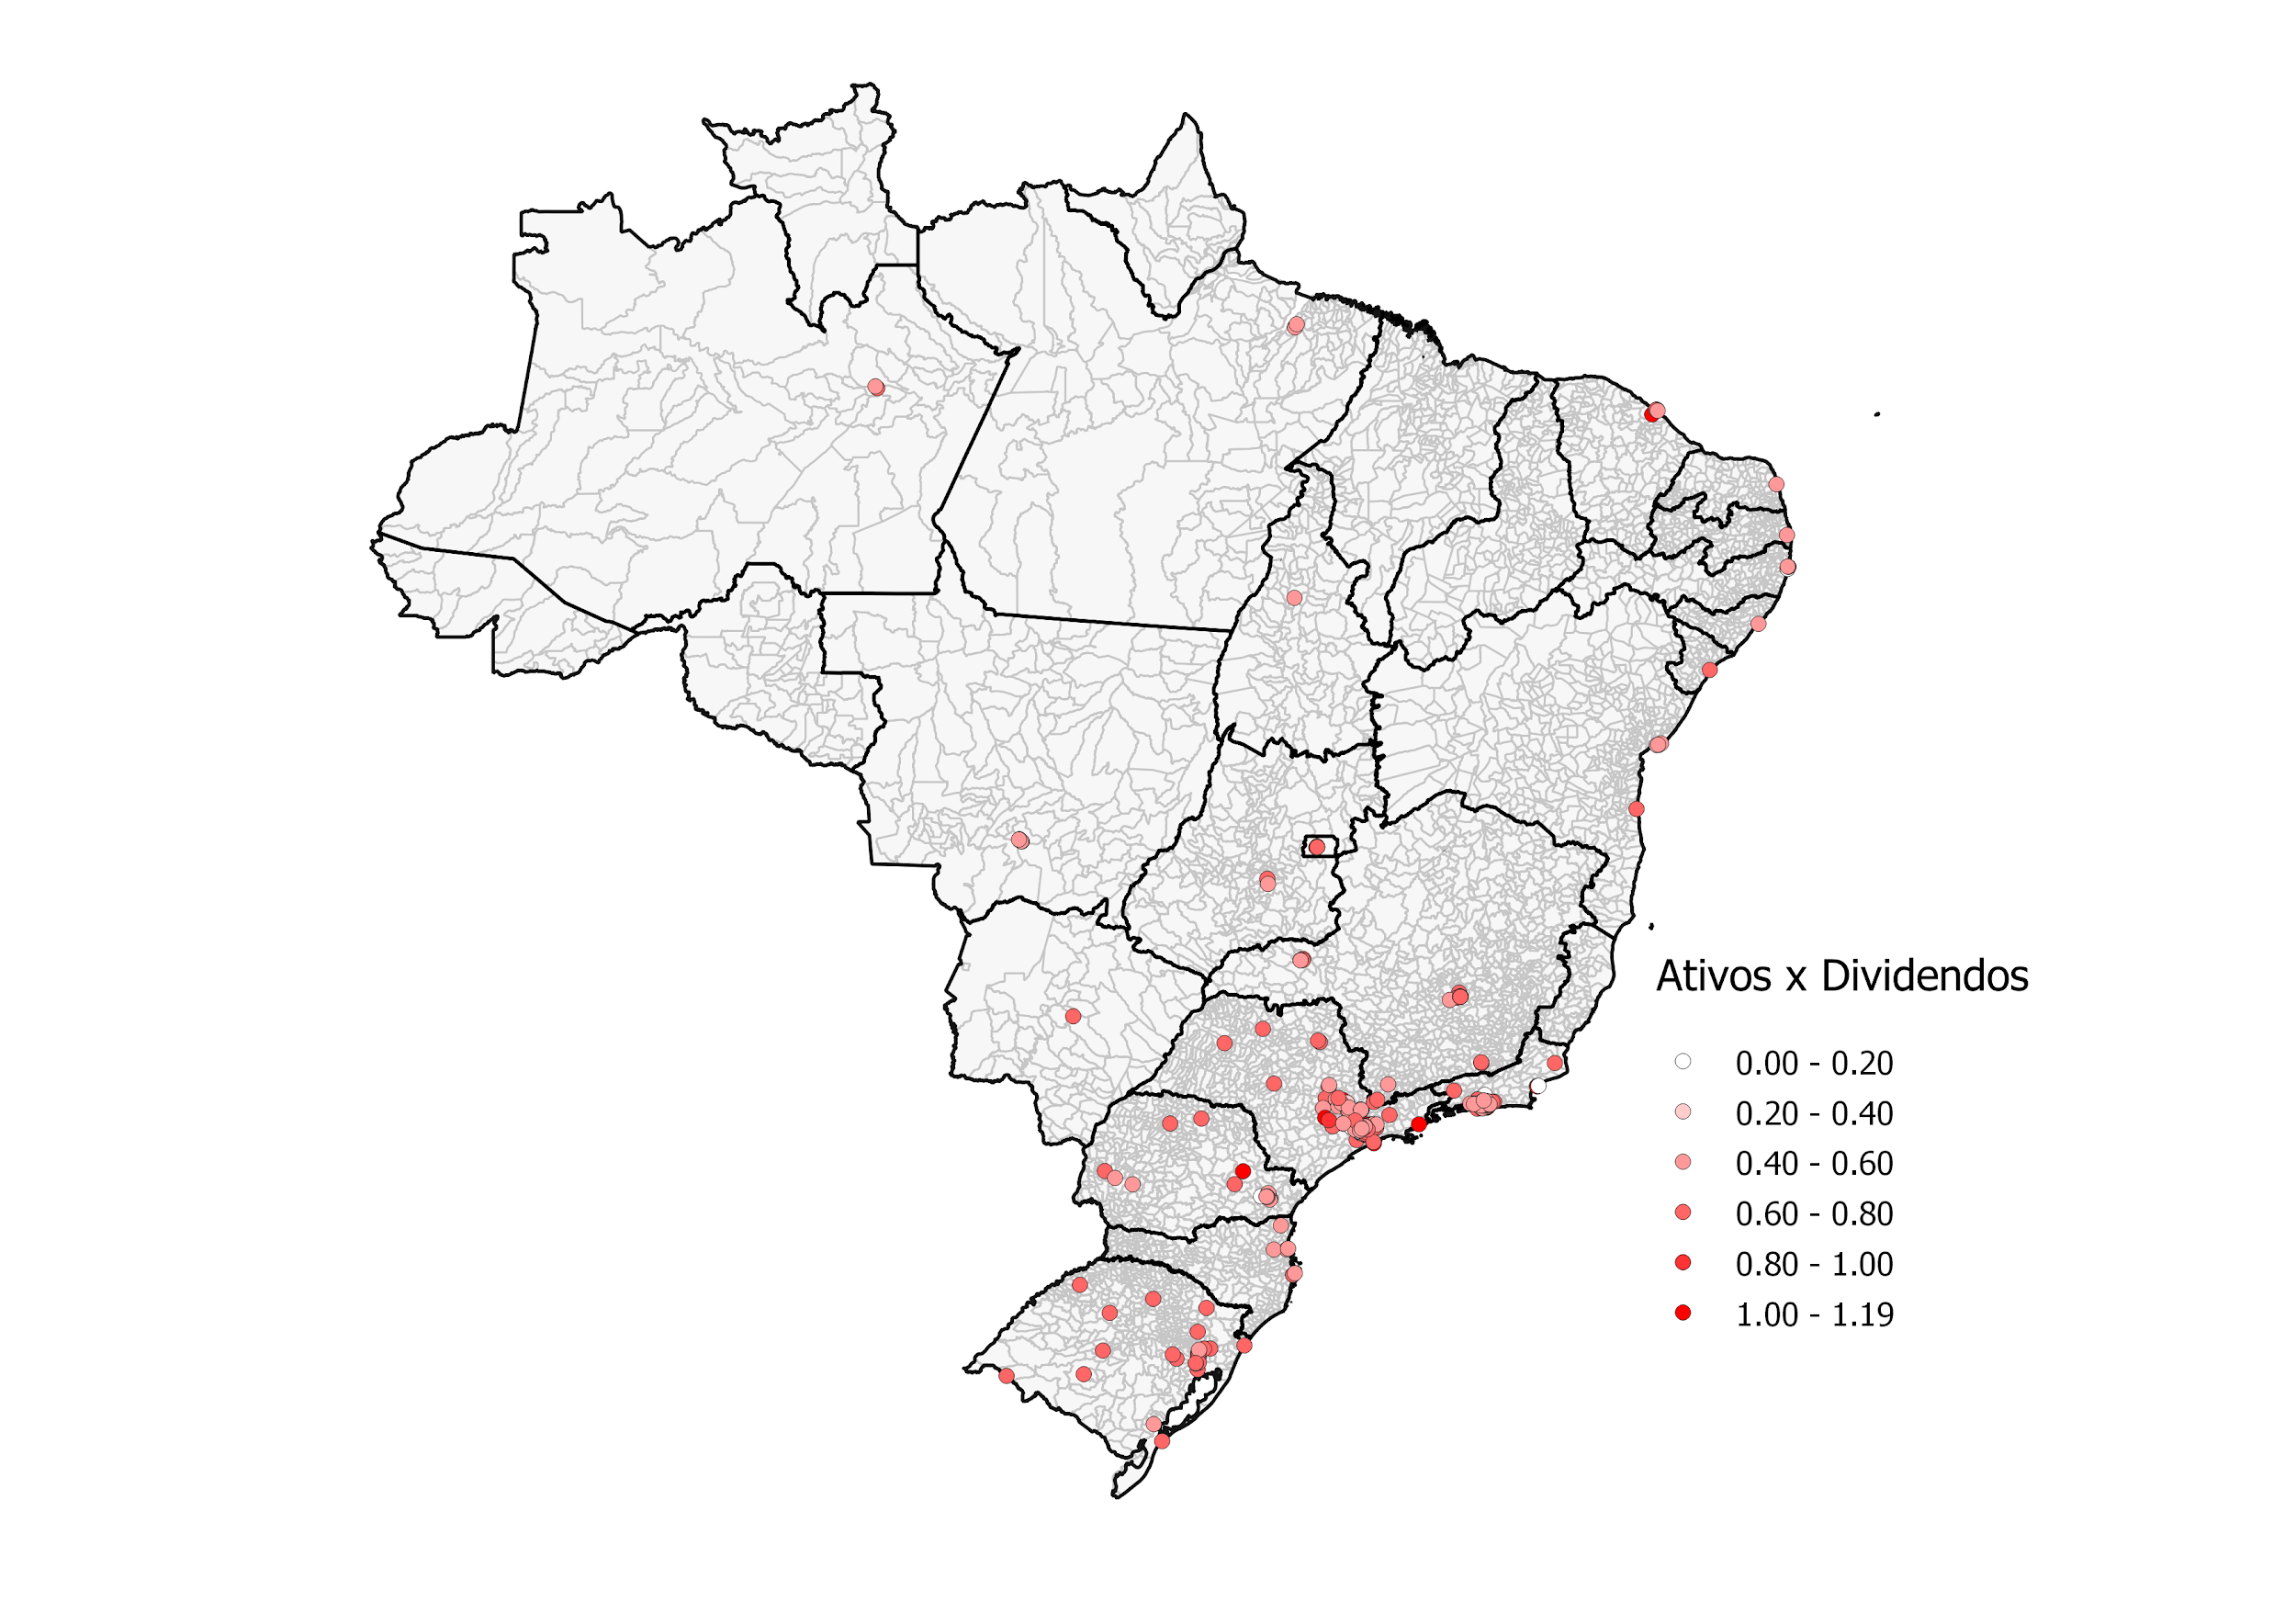
\includegraphics[width=1.0\textwidth]{AtivosxDividendosPorEstados}
\end{centering}
\caption{\label{fig:papers_vs_dividends}Os 118 ativos imobiliários em relação aos dividendos obtidos para o ano 2018/2019.}
\end{figure}
\vspace*{-44pt}
\end{center}

\begin{center}
\begin{figure}
\begin{centering}
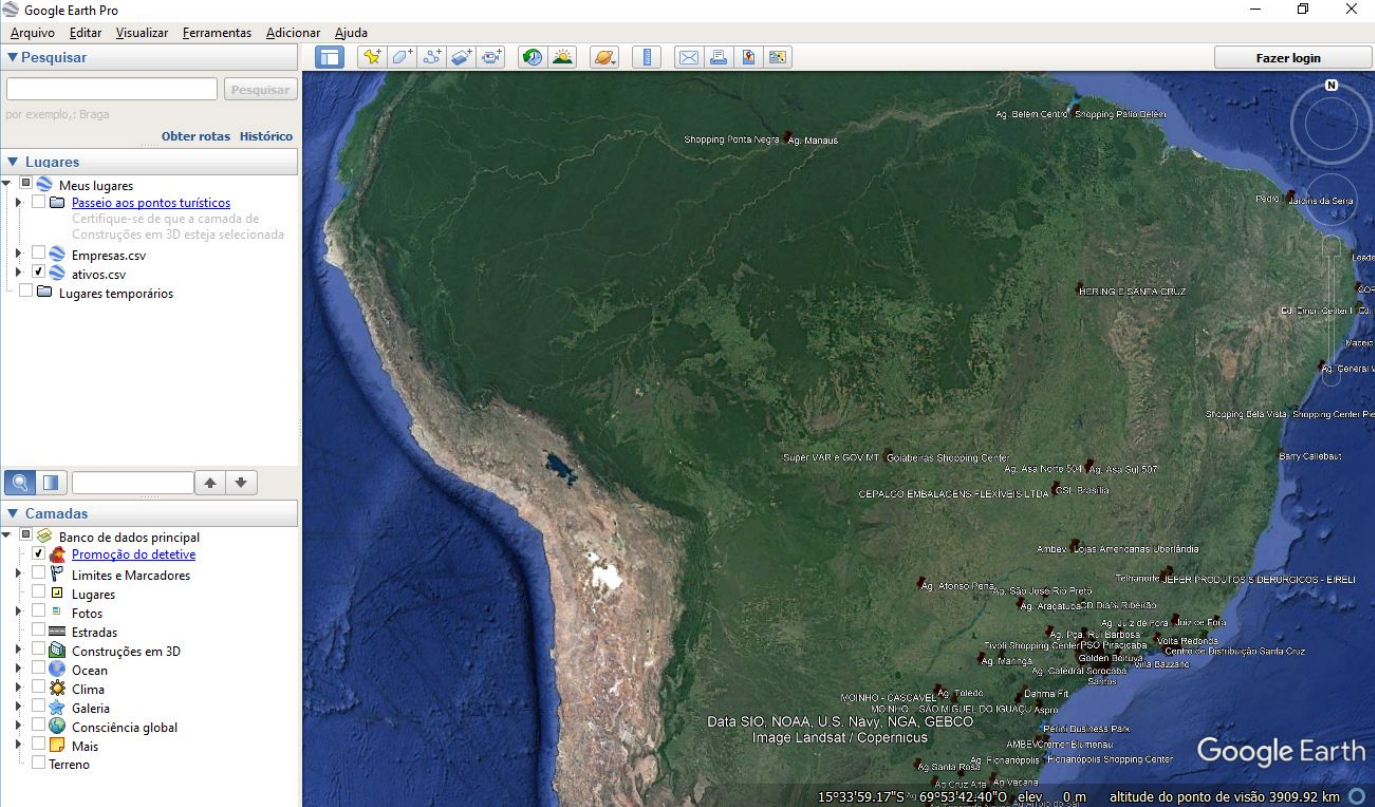
\includegraphics[width=0.85\textwidth]{GoogleEarth_Geoencoding}
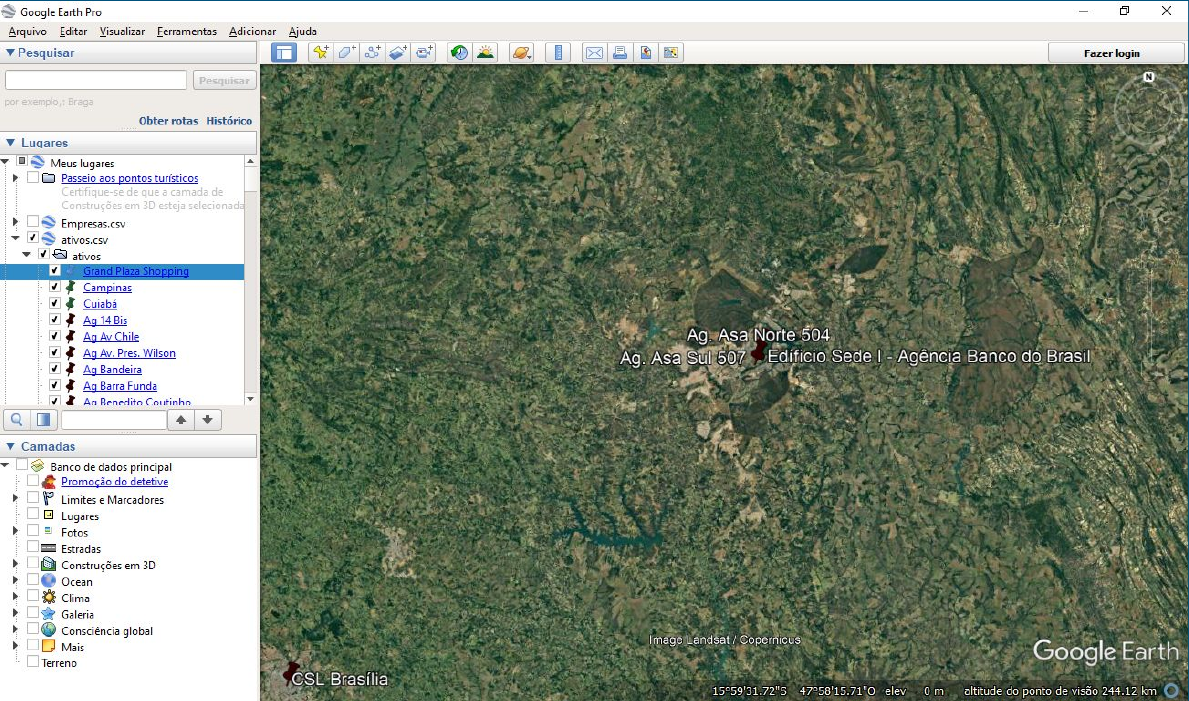
\includegraphics[width=0.85\textwidth]{GoogleEarth_GeoencodingProblems}
\end{centering}
\caption{\label{fig:geoencoding_and_problems}Processo de geocodificação no Google Earth (acima) e problemas encontrados no processamento dos endereços (abaixo).}
\end{figure}
\vspace*{-44pt}
\end{center}

O processo de geocodificação também teve seus desafios, uma vez que diversos endereços, sobretudo os da região centro-oeste, em que o Google Earth teve dificuldades de associar o endereço a uma região censitária. Um exemplo de problema de geocodificação pode ser visto na figura~\ref{fig:geoencoding_and_problems}. Logo acima, na mesma figura, encontra-se demonstrado o processo de geocodificação no Google Earth. 

Conforme mencionado, cerca de 20\% de todos os endereços apresentaram problemas. Sendo assim, foi necessário informar-se manualmente no Google Earth o endereço alvo correto.

Pode-se verificar que a maioria dos fundos se encontram-se no Sudeste e no Sul, dos fundos do sudeste, em sua maioria no estado de São Paulo, a maior concentração é no centro. No Rio Grande do Sul, os ativos estão bem espalhados, enquanto nas demais regiões do país, eles se encontram em cidades perto de cidades litorâneas. 

\begin{center}
\begin{figure}
\begin{centering}
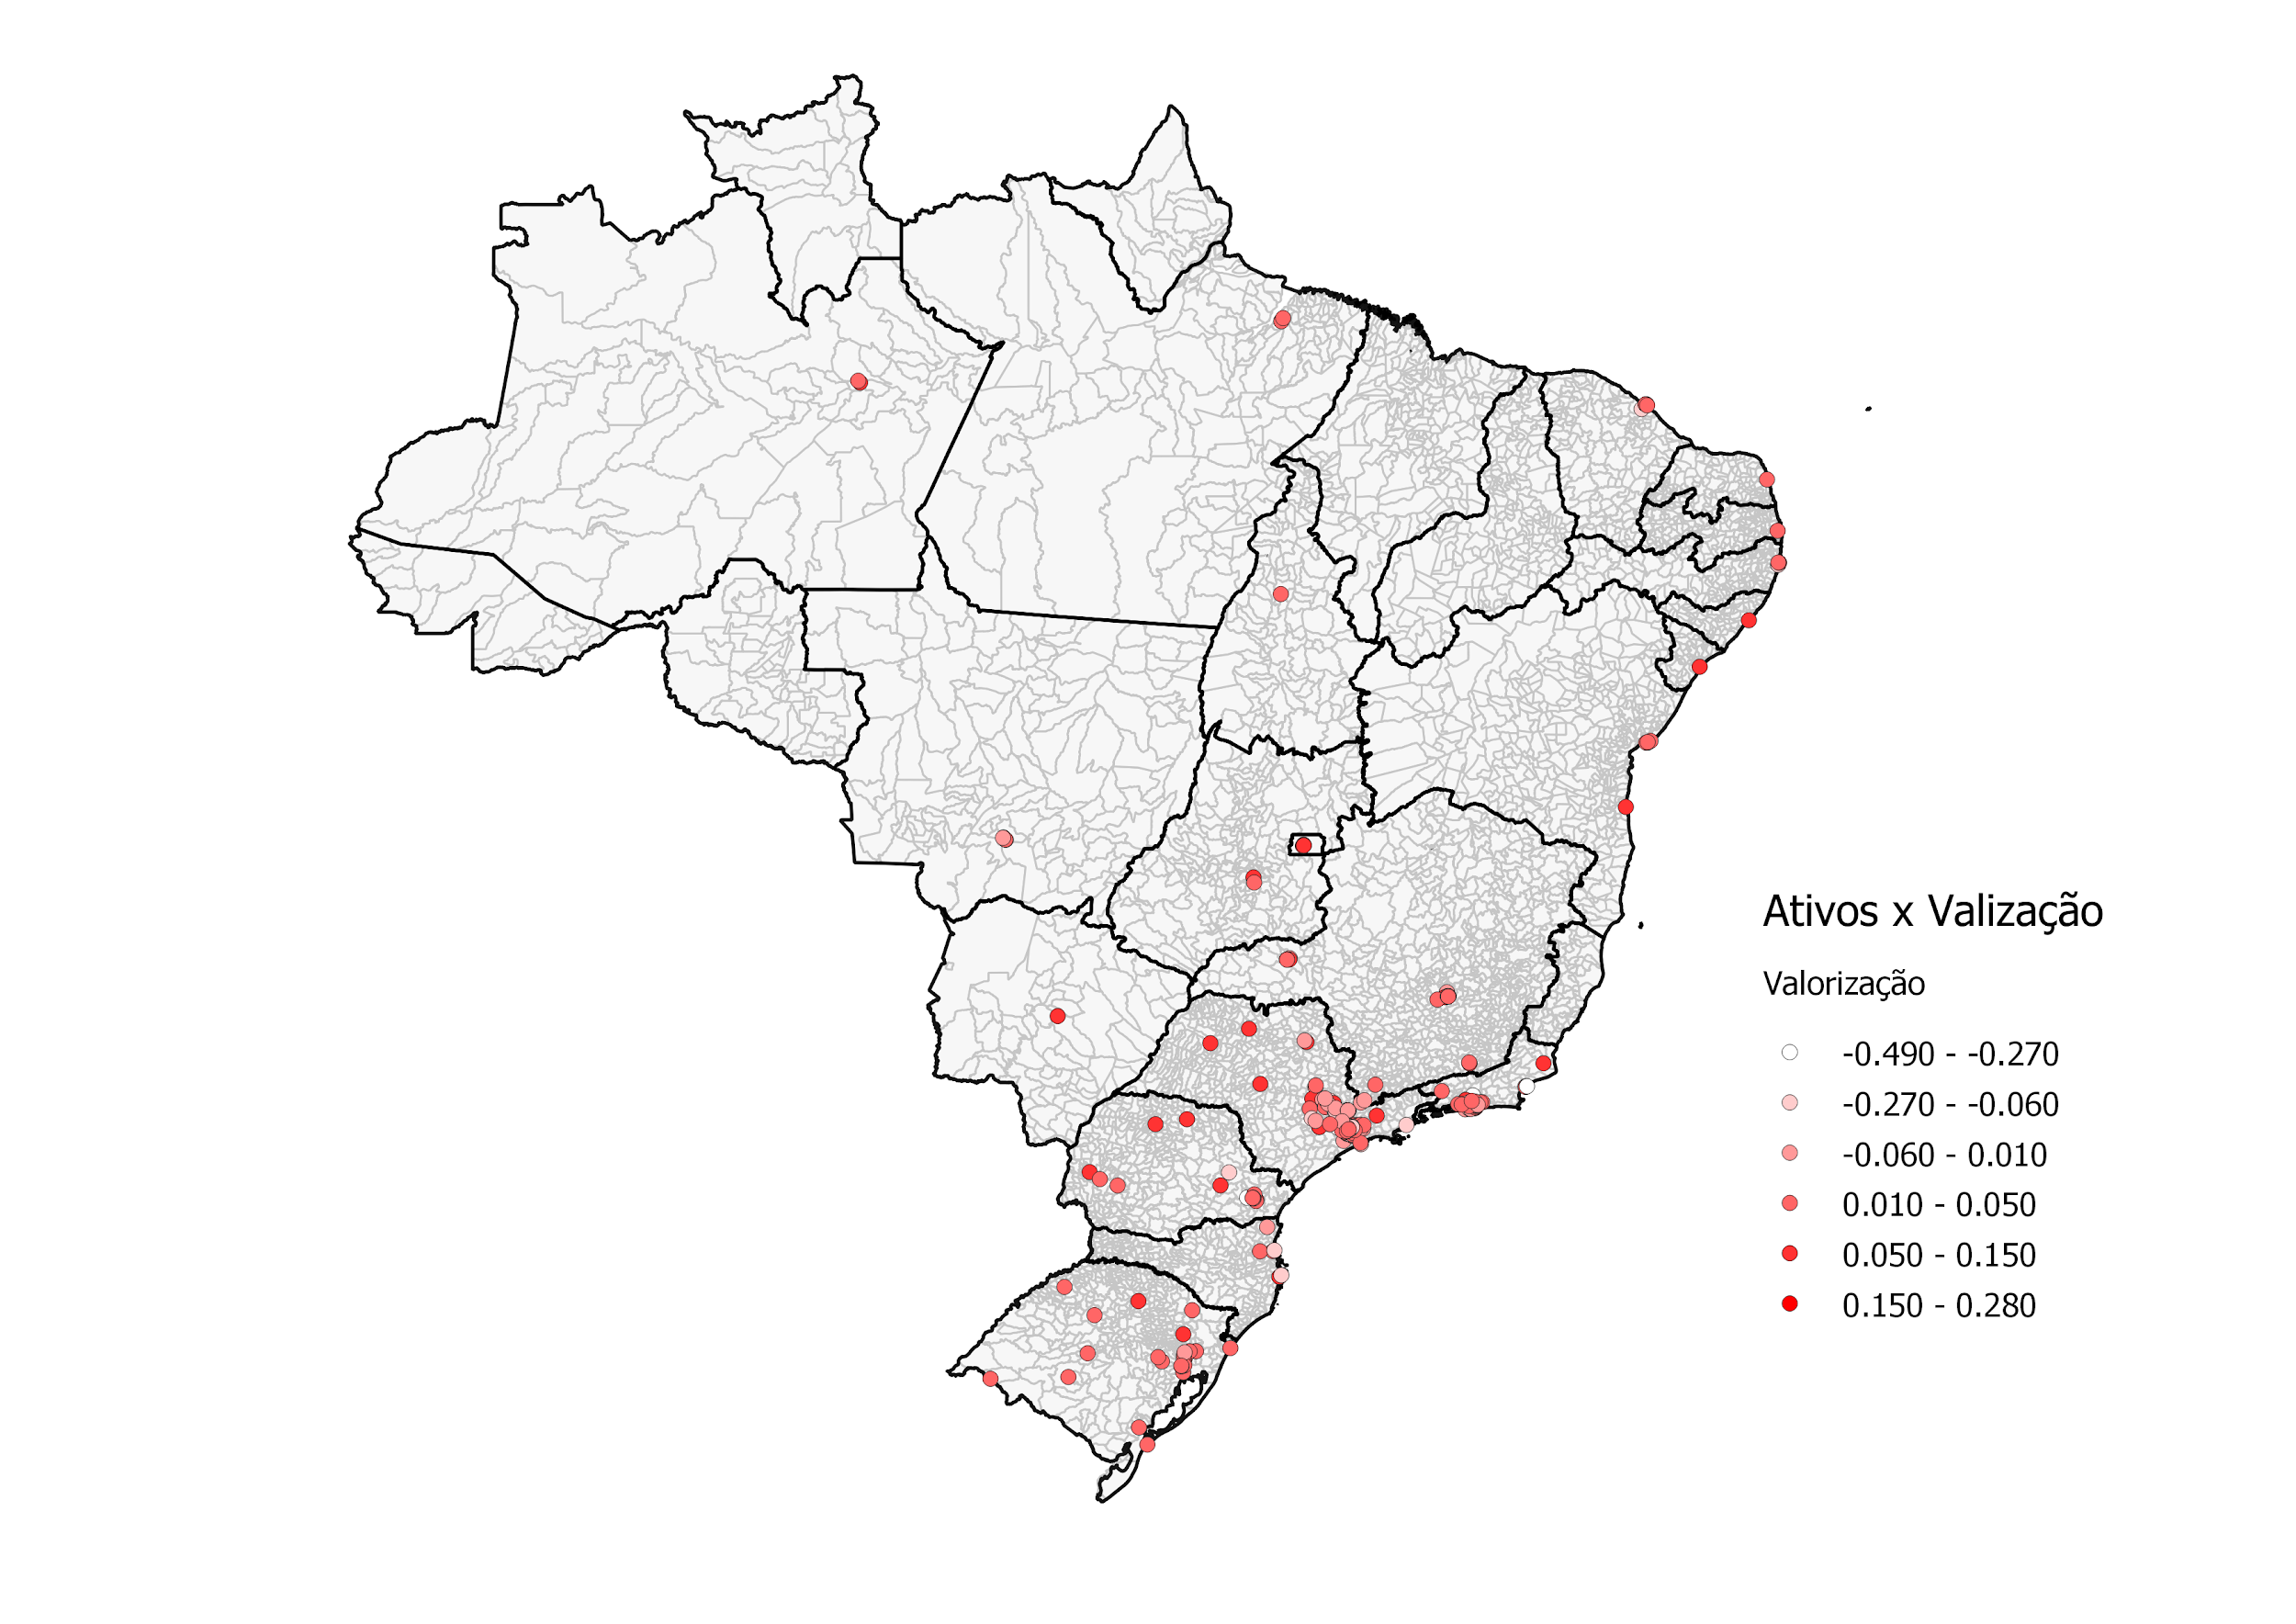
\includegraphics[width=1.0\textwidth]{AtivosxValizacaoPorEstados}
\end{centering}
\caption{\label{fig:papers_vs_valization}Os 118 ativos imobiliários em relação a valização obtida para o ano 2018/2019.}
\end{figure}
\vspace*{-44pt}
\end{center}

Esta informação casa bem com o esperado, uma vez que a concentração de pessoas e portanto de imóveis e muito maior nas cidades próximo ao litoral do que no interior do país. Nota-se também, que os fundos com maior rentabilidade são os do Sudeste, mais especificamente de São Paulo. %TODO - cite

No mapa da figura \ref{fig:papers_vs_valization}, é possível notar que existe grande correlação entre os dividendos pago pelo FII e sua valorização nos últimos 12 meses. E novamente os ativos localizado em SP, RJ e RS apresentaram maior valorização. Percebe-se assim que há uma possível relação espacial entre a localização geográfica de um ativo imobiliário e sua valorização no ano referente.

\section{Variáveis Iniciais}
\label{sec:initial_variables}
\begin{table}[h]

\begin{centering}
  \csvautobooktabular[separator=pipe]{\tablePath/VariaveisIniciais.csv}
\caption{\label{tab:initial_variables} Variáveis relacionadas aos Fundos de Investimentos Imobiliários de interesse para a análise do trabalho.}
\end{centering}
\end{table}

Na tabela \ref{tab:initial_variables}, demonstram-se as variáveis de interesse para análise, incluindo a variável localização do ativo, usada para o georeferenciamento do mesmo.

\section{Análise Multivariada}
\label{sec:multivariate_analysis}

\begin{center}
\begin{figure}
\begin{centering}
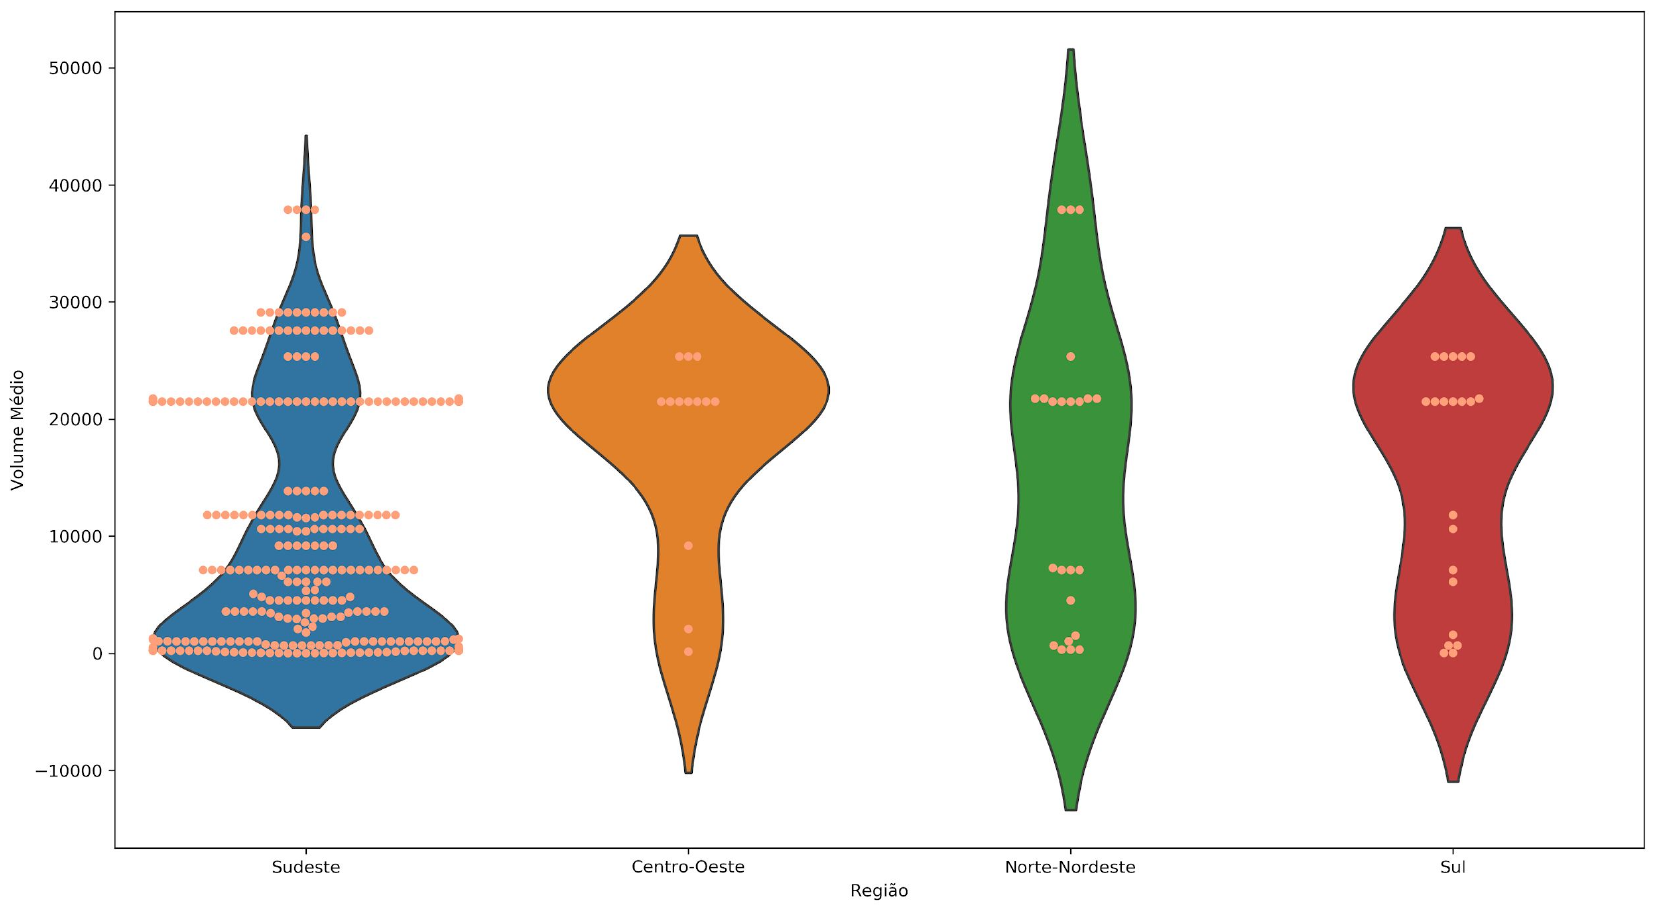
\includegraphics[width=1.0\textwidth]{RegionsPerVolume}
\end{centering}
\caption{\label{fig:regions_per_volume}Variável \emph{volume médio} por região. Observa-se no \emph{swarmplot} uma predominância de ativos com presença no Sudeste conforme esperado e visto na seção~\ref{sec:extraction_by_webscrapping}.}
\end{figure}
\vspace*{-44pt}
\end{center}

Realizamos uma análise multivariada utilizando as seguintes bibliotecas do python:

\begin{itemize}
  \item geocoder
  \item geopandas
  \item pandas
  \item pysal
  \item libpysal
  \item mapclassify
  \item seaborn
  \item matplotlib
\end{itemize}

\begin{center}
\begin{figure}
\begin{centering}
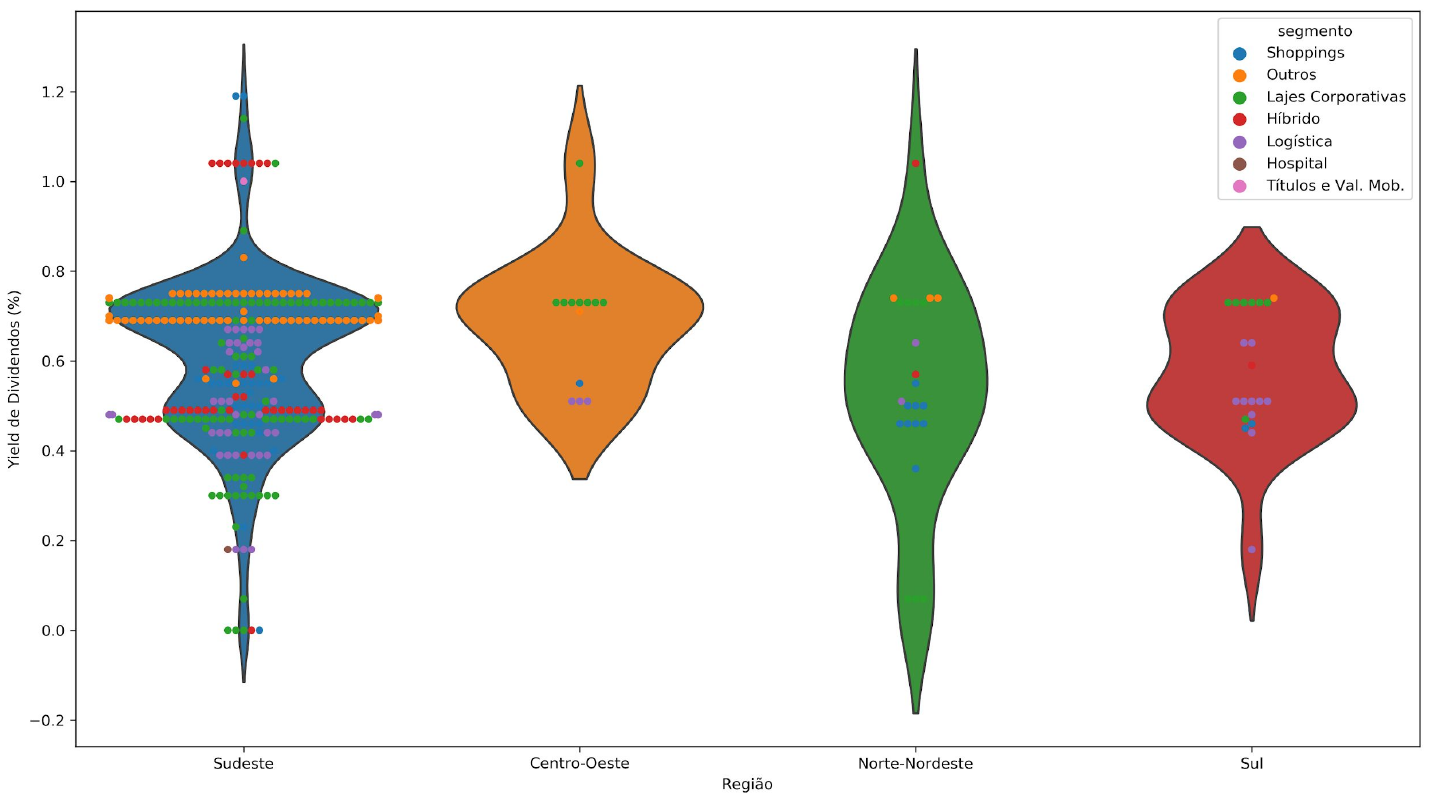
\includegraphics[width=1.0\textwidth]{RegionsPerYield}
\end{centering}
\caption{\label{fig:regions_yield}Variável \emph{yield} por região.  Os segmentos \emph{híbrido} e \emph{outros} apresentaram performance acima dos demais para a região Sudeste. Nesta mesma região \emph{lajes corporativas} possuem um retorno menor neste parâmetro.}
\end{figure}
\vspace*{-44pt}
\end{center}

Para a análise em si, inicialmente dividiu-se o Brasil nas regiões Sul, Sudeste, Centro-oeste e Norte-nordeste. Para fins de análise, tentou-se avaliar as variáveis referenciadas na seção~\ref{sec:initial_variables}. Isto é, \emph{volume médio}, $p/vp$, \emph{valorização} e \emph{yield de dividendos}.

A figura~\ref{fig:regions_per_volume} mostra o volume médio de operações mensais em relação aos ativos. Nota-se uma certa concentração de fundos sem volume, sobretudo na região \emph{Sudeste}. Isto pode ser devido tanto aos \emph{FIIs} ainda serem recentes em relação a outros investimentos mais conhecidos no mercado ou mesmo pelo fato do brasileiro não ter uma característica de investimento em papéis de maneira geral. Somente recentemente que a BOVESPA, bolsa de ações no país, passou a marca de 1 milhão de pessoas físicas cadastradas.

\begin{center}
\begin{figure}
\begin{centering}
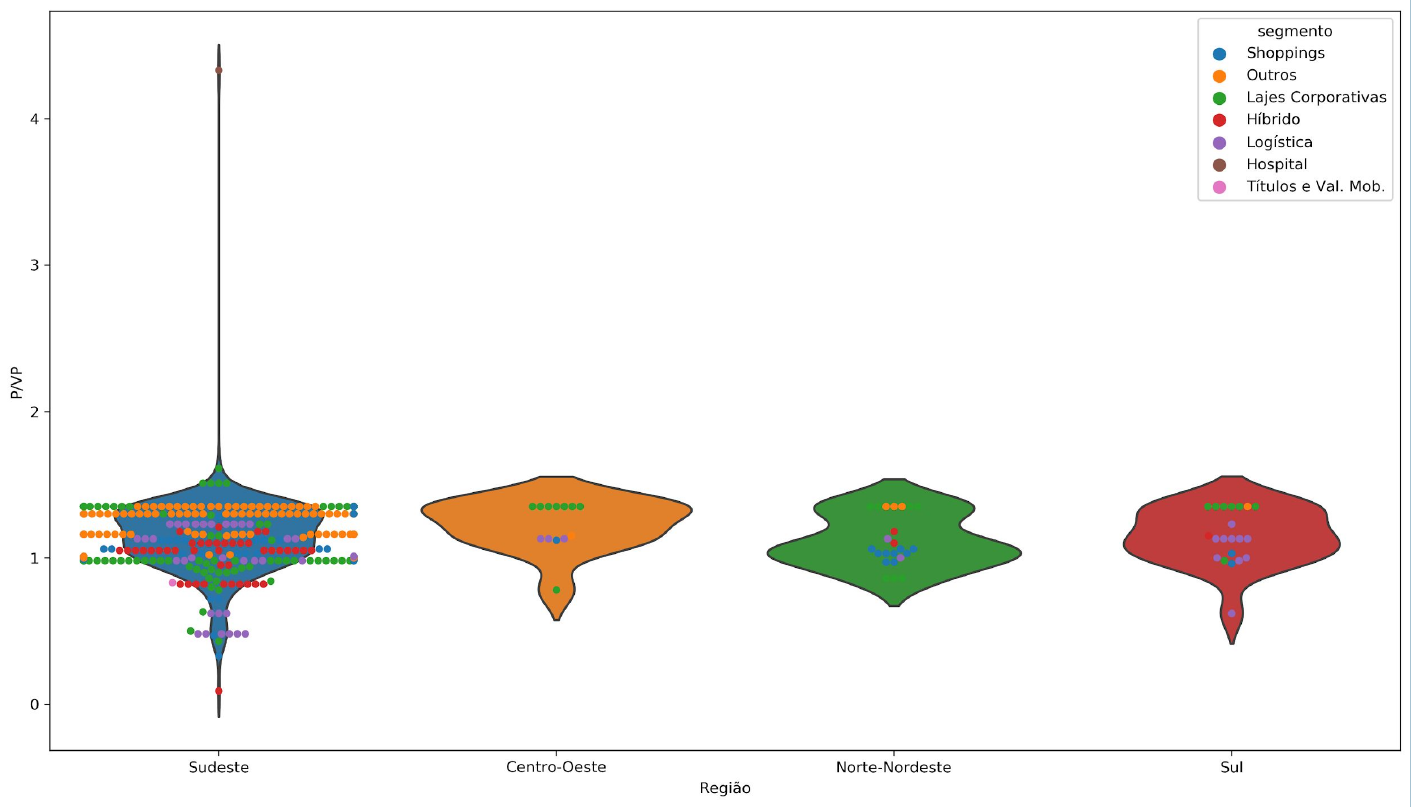
\includegraphics[width=1.0\textwidth]{RegionsPerPvp}
\end{centering}
\caption{\label{fig:regions_pvp}Variável $p/vp$ por região. Norte-nordeste é bem atrativo neste quesito.}
\end{figure}
\vspace*{-44pt}
\end{center}

Na figura~\ref{fig:regions_yield}, tem-se por cor a categoria dos fundos aos quais os ativos são pertencentes. Nota-se que na região Sudeste, mais significativa em volume de ativos, os segmentos \emph{híbrido} e \emph{outros} apresentam dividendos acima dos demais. Já \emph{lajes corporativas}, \emph{shoppings}, \emph{logística} e \emph{títulos} apresentam valores mais baixos na média. 

Com relação ao parâmetro \emph{valorização}, na figura~\ref{fig:regions_evaluation}, os segmentos que melhor desempenham são \emph{lajes corporativas} e \emph{outros}. Para a região centro-oeste, a primeira também apresenta valorização significativa.

\begin{center}
\begin{figure}
\begin{centering}
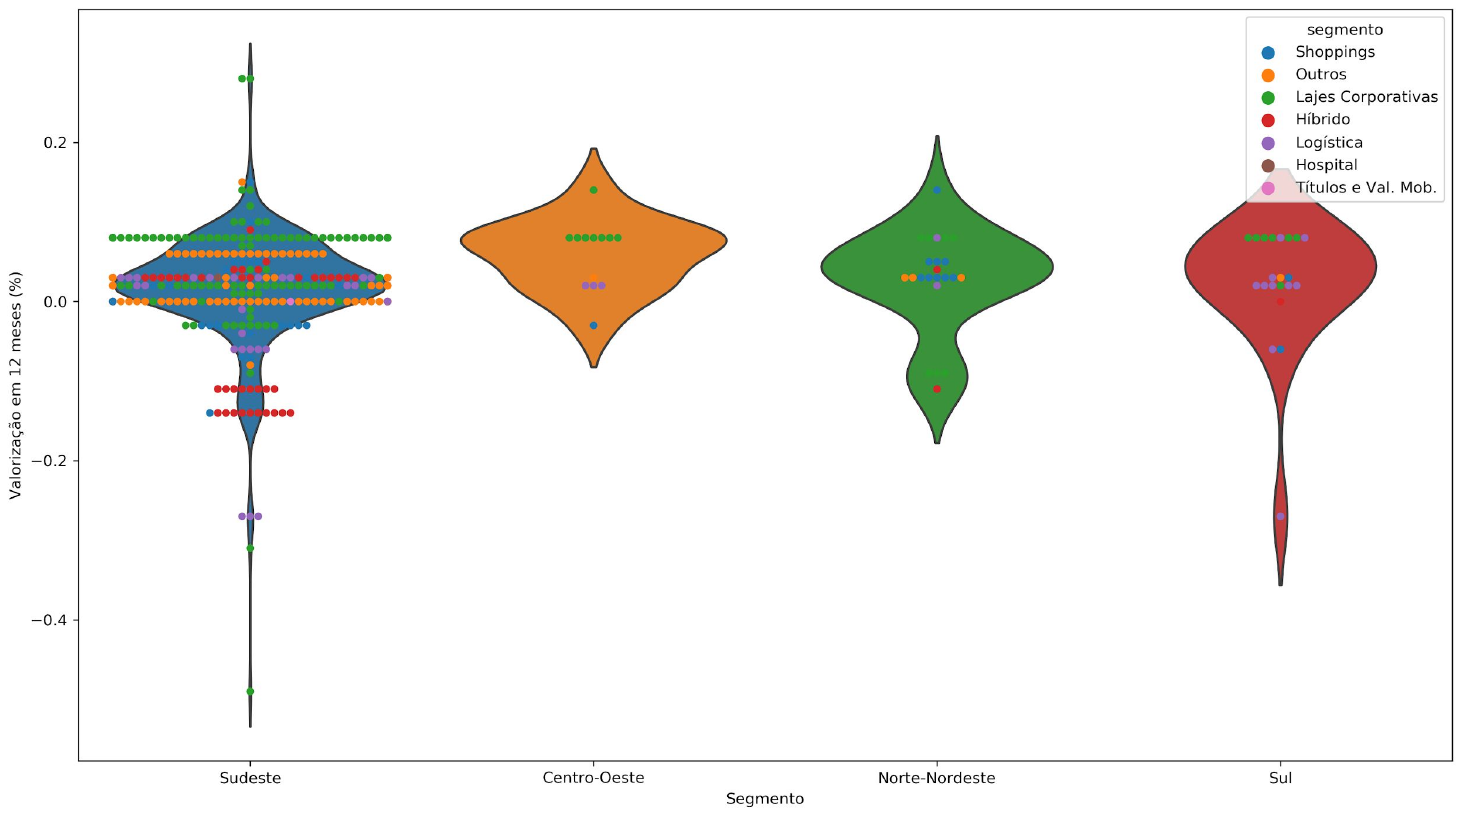
\includegraphics[width=1.0\textwidth]{SegmentPerEvaluation}
\end{centering}
\caption{\label{fig:regions_evaluation}Variável \emph{valorização} por região (12 meses). Observa-se no \emph{swarmplot} uma predominância de ativos com presença na região Sudeste.}
\end{figure}
\vspace*{-44pt}
\end{center}

Por fim, nota-se na figura~\ref{fig:regions_pvp}, que é uma variável tipicamente presente em análises fundamentalistas, onde valores acima de 1 significam valorização acima do esperado (preço alto) e valores abaixo de 1, preço baixo. Pela análise desta variável o setor de \emph{lajes corporativas}, \emph{híbrido} e \emph{logística} despontam como mais interessantes para compra na região sudeste. nas demais regiões observa-se forte valorização do preço das \emph{lajes corporativas}.

\section{Análise Espacial}
\label{sec:spatial_analysis_br}

A análise espacial de pesos é feita a partir da resolução da matriz de pesos da vizinhança de uma variável qualquer num grid regular espaçado em um quadrado \emph{n por n}. O grid $W$ é dado pela razão dos pesos dos seus vizinhos, isto é:

\[
W_{nxn}=\left[\begin{array}{cccc}
w_{11} & w_{12} & ... & w_{1n}\\
w_{21} & w_{22} & ... & w_{2n}\\
... & ... & ... &...\\
w_{n1} & w_{n2} & ... & w_{nn}
\end{array}\right]
\]

Para a matriz de pesos \emph{Queen}, de grau 1, cada peso é calculado a partir da vizinhança imediata cheia, isto é os 8 elementos adjacentes. Já o método de \emph{Rock}, prevê somente aquelas adjacentes ortogonalmente, mas não aquelas em que a adjacência seja diagonal ao elemento, isto é, em formato de cruz.

\begin{center}
\begin{figure}
\begin{centering}
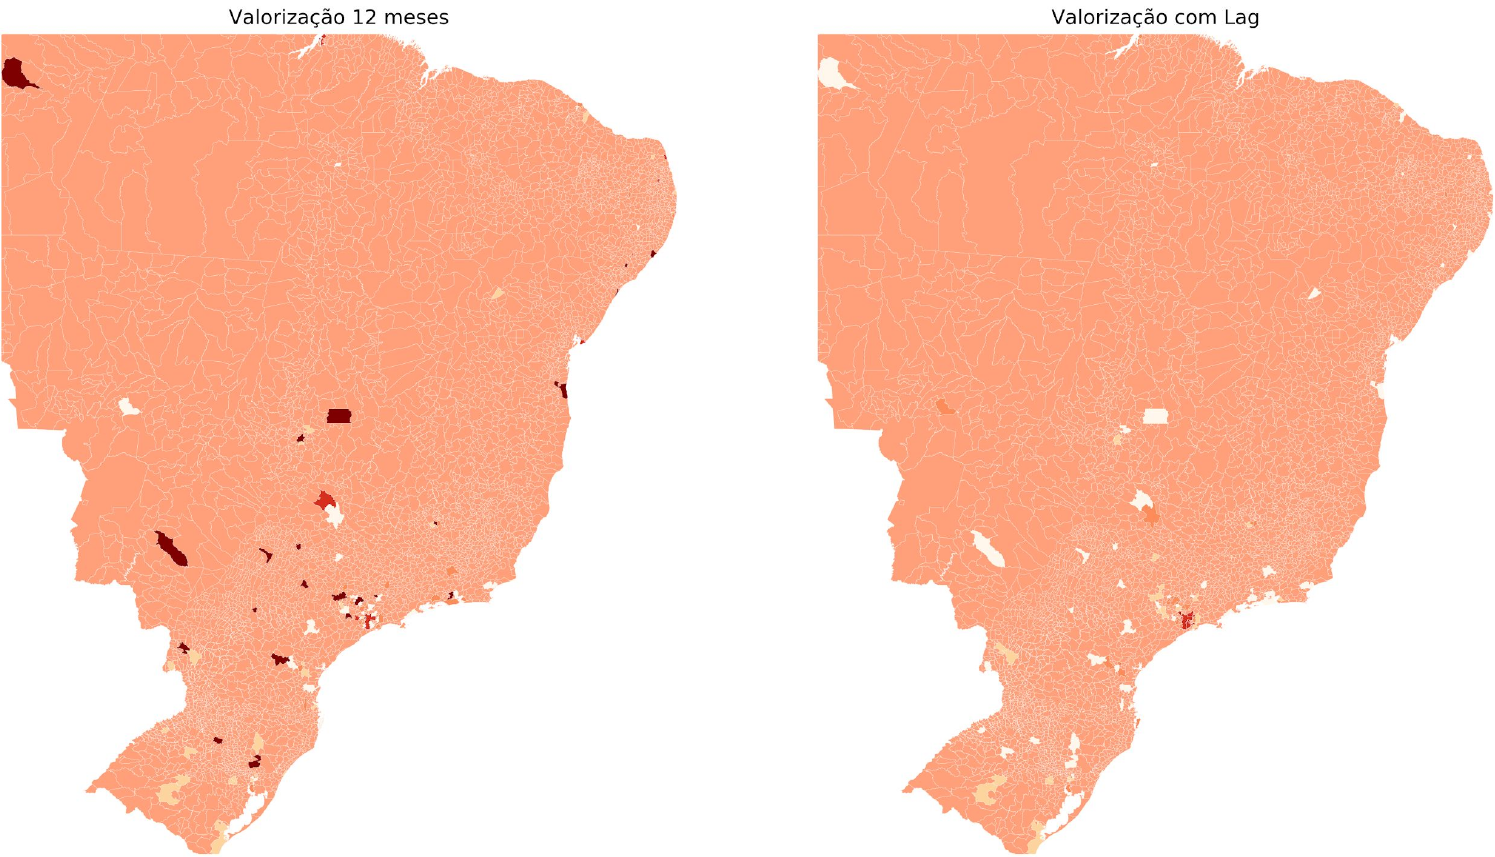
\includegraphics[width=1.0\textwidth]{EvaluationPerCensitaryRegions}
\end{centering}
\caption{\label{fig:brazil_evaluation}Valorização com relação as regiões censitárias. Do lado esquerdo a valorização absoluta e do lado direito a valorização levando em consideração a vizinhança por Queen com $n=1$ de lag.}
\end{figure}
\vspace*{-44pt}
\end{center}

Os pesos são calculados amostrando-se pelos chamados \emph{pesos padronizados por linha}, segundo a fórmula:

\[
w_{ij(s)}=w_{ij}/\sum_{j}w_{ij}
\]

Um outro fator importante já mencionado é a contiguidade que apresenta formas diferentes para o método de \emph{Queen} e \emph{Rock}. Ambos métodos são extremamente sensíveis ao fator de continuidade dos dados e por isso caso não haja um casamento adequado aos dados, é possível que seja necessário tratá-los.

\begin{center}
\begin{figure}
\begin{centering}
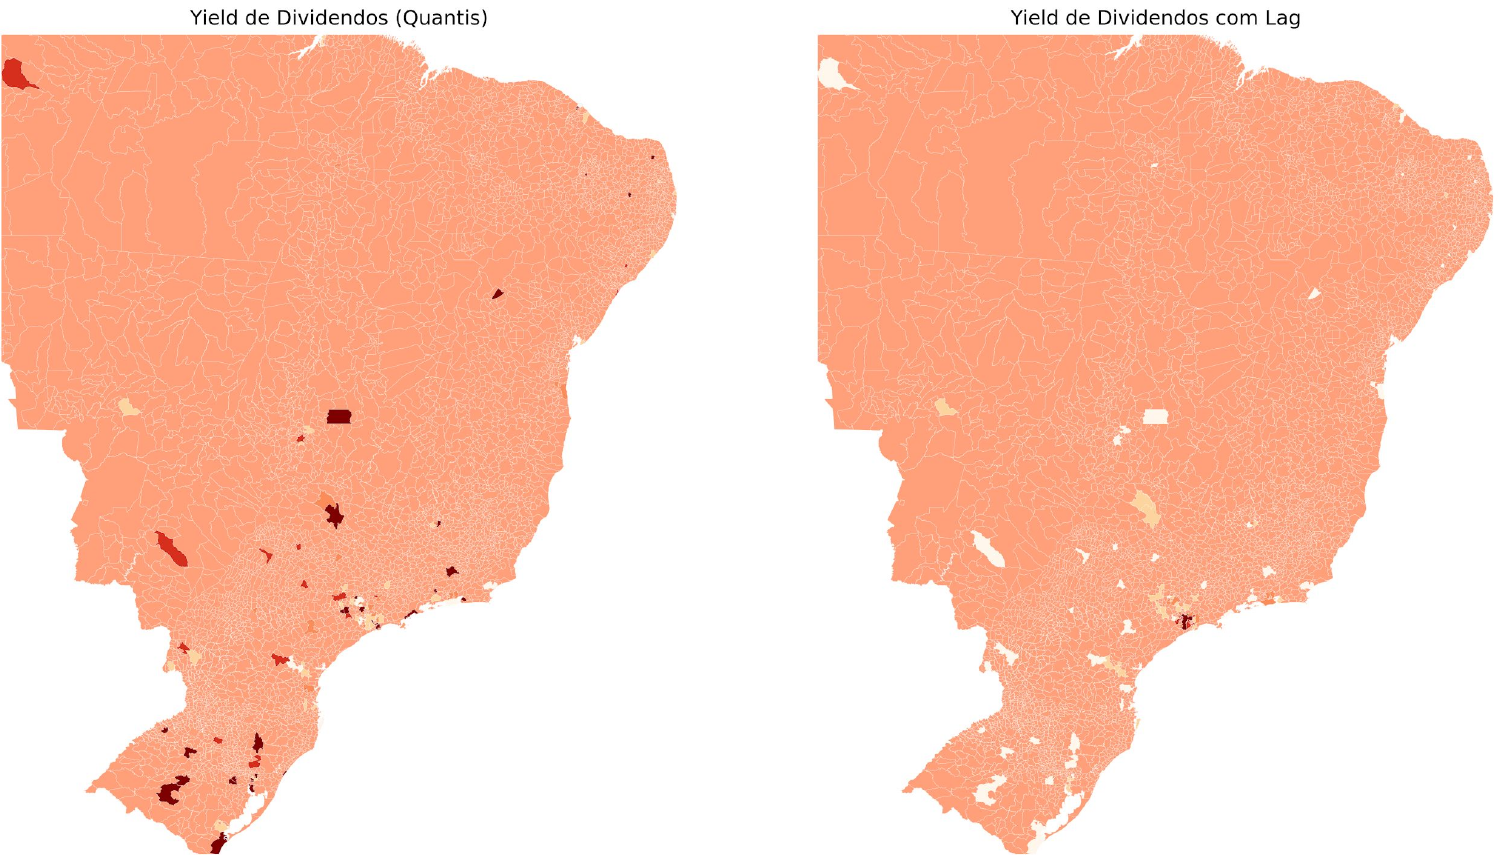
\includegraphics[width=1.0\textwidth]{YieldPerCensitaryRegionWithlag}
\end{centering}
\caption{\label{fig:brazil_yields}\emph{Yield} com relação as regiões censitárias. Do lado esquerdo a valorização absoluta e do lado direito a valorização levando em consideração a vizinhança por Queen com $n=1$ de lag.}
\end{figure}
\vspace*{-44pt}
\end{center}

As figuras~\ref{fig:brazil_evaluation} e~\ref{fig:brazil_yields} demonstram a \emph{valorização} e o \emph{yield} de cada ativo por região censitária. Em ambos os casos somente a região de São Paulo capital ainda permance com um valor significativo levando-se em consideração a vizinhança. 

Conforme mencionado anteriormente, a análise de pesos por Queen é muito sensível a densidade de dados da vizinhança. Sendo assim, decidiu-se reduzir o escopo dos ativos àqueles da região da capital paulista somente.

\section{Análise Espacial de São Paulo}
\label{sec:spatial_analysis_sao_paulo}

\begin{center}
\begin{figure}
\begin{centering}
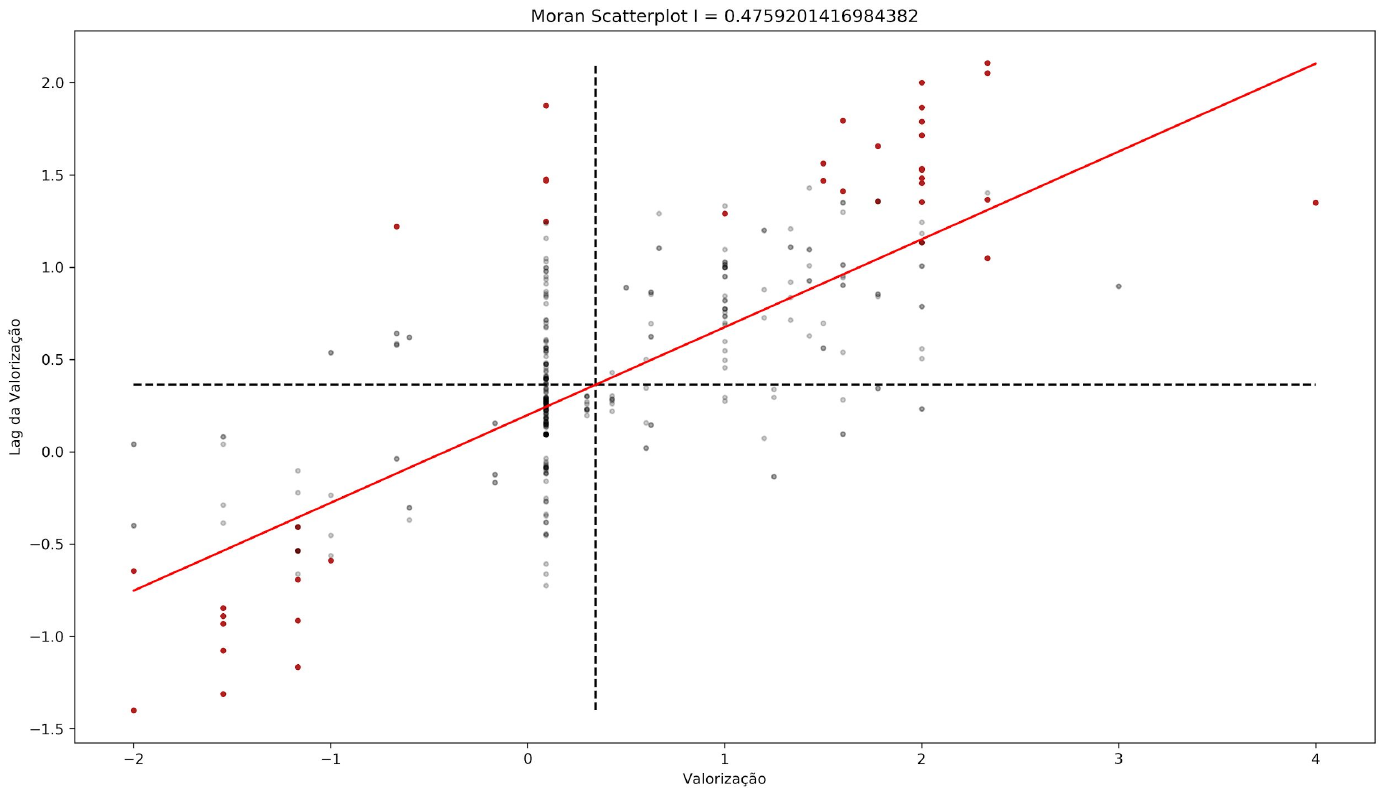
\includegraphics[width=1.0\textwidth]{MoranI}
\par\end{centering}
\caption{\label{fig:moran_i} I de Moran para a valorização em relação ao lag da mesma.} 
\end{figure}
\vspace*{-44pt}
\end{center}

\begin{table}
\begin{lstlisting}[basicstyle={\scriptsize},tabsize=4]
REGRESSION
----------
Data set            :  sao_paulo_renda
SUMMARY OF OUTPUT: ORDINARY LEAST SQUARES ESTIMATION
Dependent Variable  :       RENDA  Number of Observations:  524
Mean dependent var  :     2368.22  Number of Variables   :    2
S.D. dependent var  :      1852.5  Degrees of Freedom    :  522 

R-squared           :    0.027862  F-statistic           :     14.9608
Adjusted R-squared  :    0.026000  Prob(F-statistic)     :  0.00012364
Sum squared residual:1.74813e+009  Log likelihood        :    -4678.85
Sigma-square        :3.34891e+006  Akaike info criterion :      9361.7
S.E. of regression  :        1830  Schwarz criterion     :     9370.22
Sigma-square ML     :3.33613e+006
S.E of regression ML:     1826.51

-----------------------------------------------------------------------------
       Variable      Coefficient      Std.Error    t-Statistic   Probability
-----------------------------------------------------------------------------
          CONSTANT       2326.63        80.6639        28.8436     0.00000
        valorizaca         14432        3731.21        3.86792     0.00012
-----------------------------------------------------------------------------

REGRESSION DIAGNOSTICS  
MULTICOLLINEARITY CONDITION NUMBER   1.143500
TEST ON NORMALITY OF ERRORS
TEST                  DF           VALUE             PROB
Jarque-Bera            2           518.2554          0.00000

RANDOM COEFFICIENTS
DIAGNOSTICS FOR HETEROSKEDASTICITY  
TEST                  DF           VALUE             PROB
Breusch-Pagan test     1             3.9064          0.04810
Koenker-Bassett test   1             1.4837          0.22319
============================== END OF REPORT ================================
\end{lstlisting}

\caption{\label{tab:regression_result} Resultado da regressão de renda em relação a variável valorização.}
\end{table}

\begin{center}
\begin{figure}
\begin{centering}
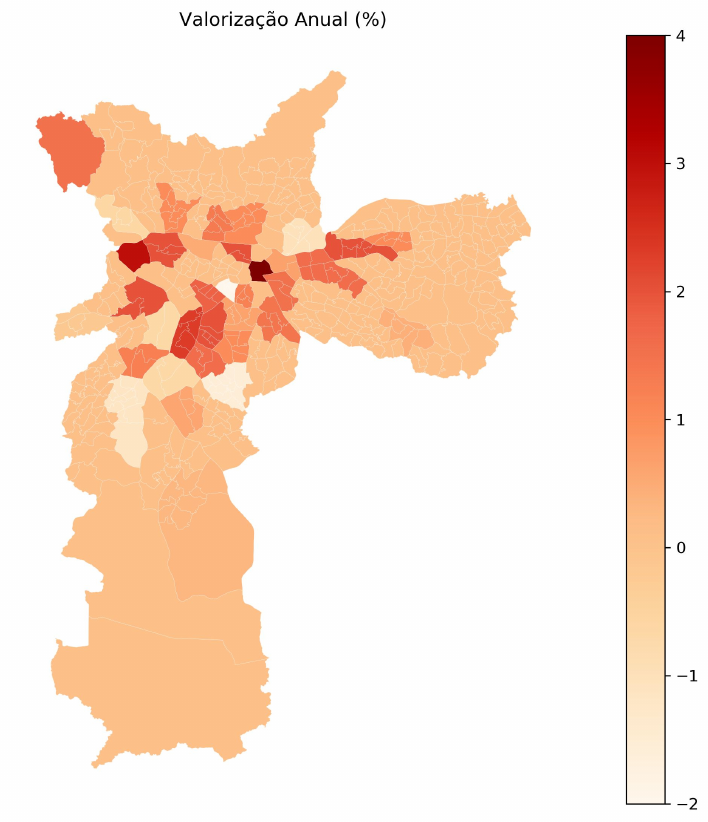
\includegraphics[width=.49\textwidth]{SaoPauloEValuationRegions}
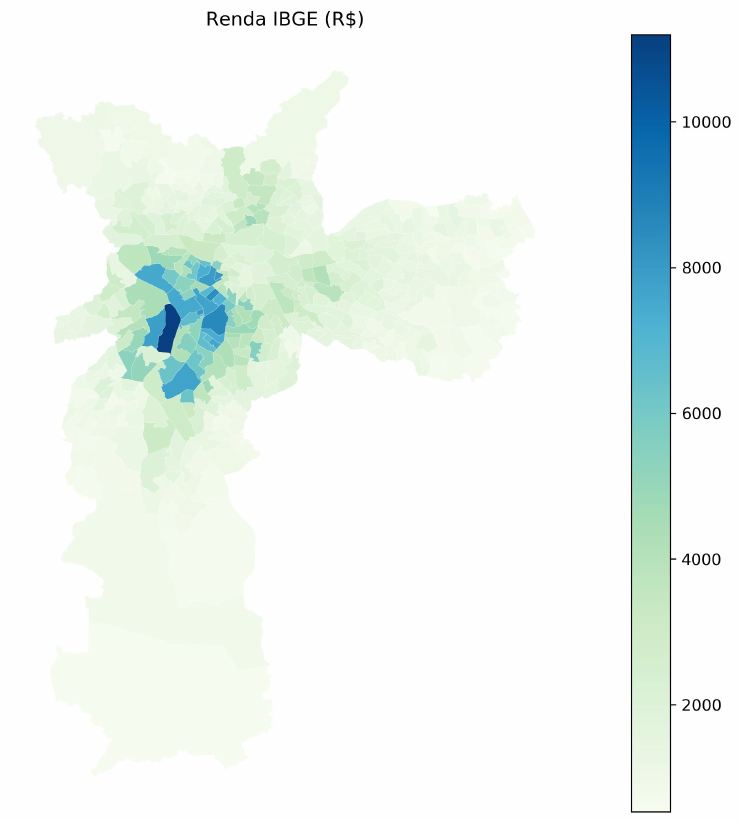
\includegraphics[width=.49\textwidth]{SaoPauloAvgIncome}
\end{centering}
\caption{\label{fig:sao_paulo_stats} À esquerda, o gráfico de valorização na cidade de São Paulo e à direita, o gráfico de salário médio para as regiões censitárias da capital do estado de São Paulo.}
\end{figure}
\end{center}

\begin{center}
\begin{figure}
\begin{centering}
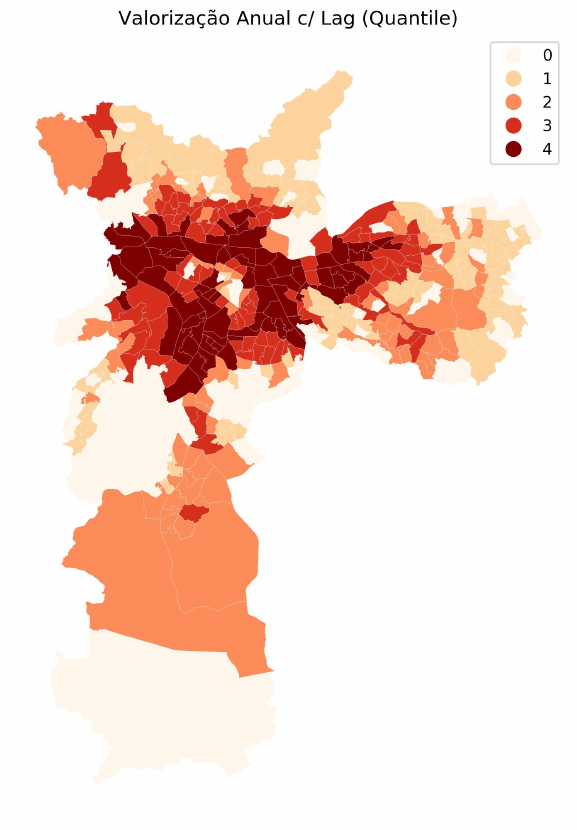
\includegraphics[width=0.6\textwidth]{SaoPauloEvaluationRegionsWithLag}
\par\end{centering}
\caption{\label{fig:sao_paulo_evaluation_with_lag} Valorização anual com lag e vizinhança $n=1$ (Queen). Na legenda apresenta-se a escala em quartis.} 
\end{figure}
\vspace*{-44pt}
\end{center}

A figura~\ref{fig:sao_paulo_stats} mostra tanto o gráfico de valorização anual dos imóveis como os dados censitários do IBGE para as regiões da capital paulistana. Diversas das regiões com renda mais acentuada são também regiões onde a valorização anual dos imóveis se destacou. Sendo assim, é possível entender-se que há uma certa relação intrínseca entre as duas variáveis.

Na figura~\ref{fig:sao_paulo_evaluation_with_lag}, nota-se uma certa difusão ou espalhamento dos efeitos observados na figura~\ref{fig:sao_paulo_stats}. Sendo assim, há para a cidade de São Paulo uma certa razão para os fatores observados.

\subsection{Relação entre Renda e Valorização}
\label{sec:income_evaluation}
Sendo assim observada a relação, será possível traçar-se a relação entre as duas variáveis observadas?

Na tabela~\ref{tab:regression_result}, demonstra-se o resultado da regressão de renda para variável. Nota-se que o $R^{2}$ observado é muito pequeno indicando pouquíssima ou nenhuma correlação. Isto deve-se ao fato, observado na seção~\ref{sec:multivariate_analysis}, que os fundos possuem ativos em diversos distritos e inclusives em diversos estados. 

No caso desta seção, os mesmos fundos possuem ativos em diversos setores de São Paulo, o que implica que o índice final apresentado não é por imóvel, mas sim por fundo. 

Distritos com somente um fundo vão apresentar a valorização do mesmo. Ou seja, é provável que esteja-se alterando o valor esperado do imóvel na região ao analisar-se a performance do fundo em si. 

Para que fosse possível fazer uma análise completa da performance por imóvel, seria interessante acessar o valor base, por imóvel, que compõe o índice final de valorização de cada fundo. Infelizmente, esta informação não está prontamente disponível para utilização nas fontes utilizadas para a extração.

Por fim, a figura~\ref{fig:moran_i}, mostra o I de Moran para a valorização em relação ao seu lag das figuras~\ref{fig:sao_paulo_evaluation_with_lag} e~\ref{fig:sao_paulo_stats}. Este I, apesar de indicar que há correlação espacial também mostra a tendência mencionada anteriormente, na qual diversos distritos, em localizações distintas possuem índices parecidos em função da granularidade dos dados serem por fundo e não por ativo.
